\subsubsection{Attività}
	\paragraph{Verifica di un ticket}
	Ogni qual volta un ticket sarà contrassegnato come \textbf{Completato} il \RES procederà nel seguente modo: 
	\begin{itemize}
		\item crea un ticket di verifica;
		\item lo assegna ad un \textbf{verificatore};
		\item non appena il ticket viene contrassegnato come \textbf{Completato} imposta il tag del ticket oggetto di verifica a \textbf{Verificato}.
	\end{itemize}
	\begin{figure}
		\centering
		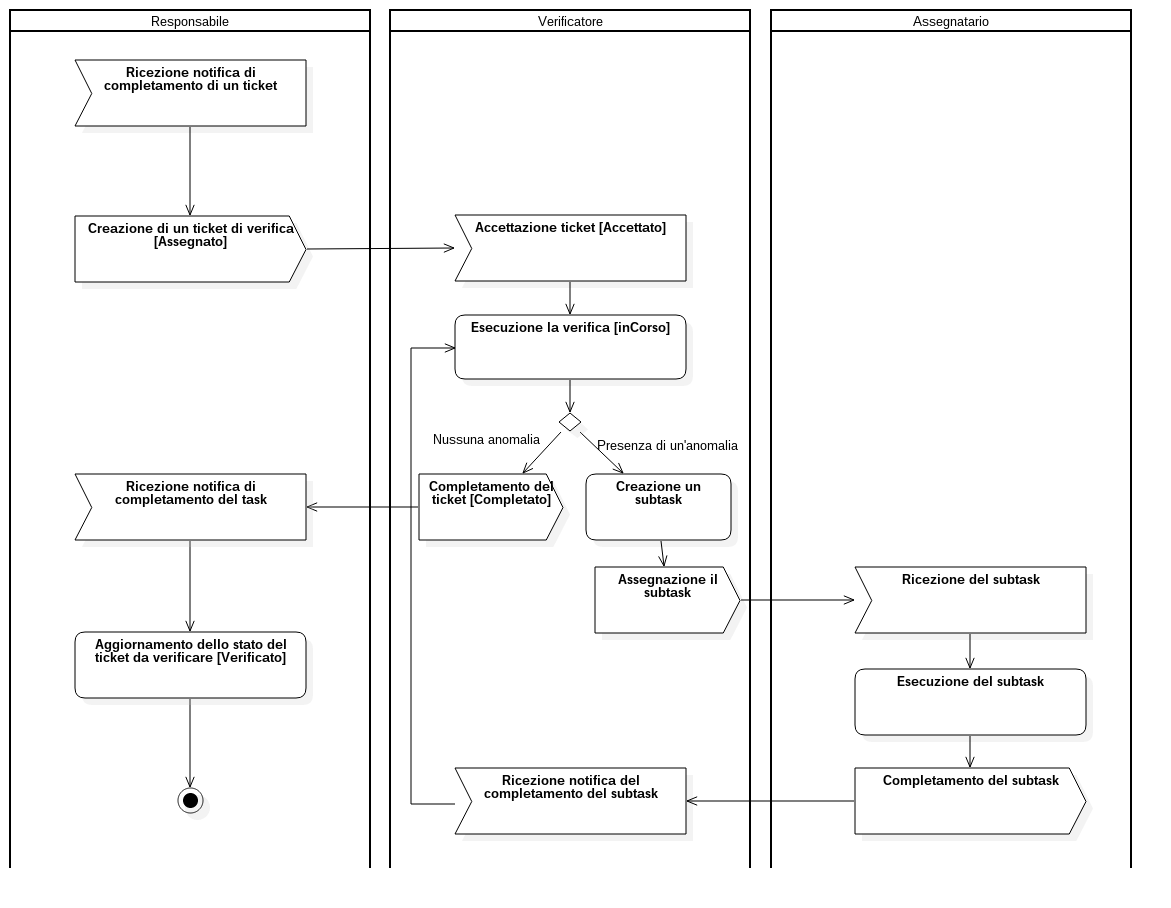
\includegraphics[scale=0.40]{img/ticketVerifica.png}
		\caption{Ticket di verifica}
	\end{figure}
\subsubsection{Procedure}
	\paragraph{Gestione delle anomalie}
			Il \textbf{validatore} qualora riscontrasse delle anomalie procederà secondo la seguente procedura:
			\begin{itemize}
				\item crea un nuovo subtask del ticket di verifica per ogni anomalia riscontrata;
				\item assegna un titolo breve e preciso ad ogni subtask;
				\item se necessario aggiunge un commento che descriva l'anomalia riscontrata;
				\item assegna i subtasks al redattore del documento.
			\end{itemize}